S\-W\-E is a teaching code that implements simple Finite Volumes models that solve the shallow water equations -\/ in a problem setting as it would be used for tsunami simulation.\hypertarget{index_intro}{}\section{The Shallow Water Equations}\label{index_intro}
The shallow water equations describe the behaviour of a fluid, in particular water, of a certain (possibly varying) depth {\itshape h} in a two-\/dimensional domain -- imagine, for example, a puddle of water or a shallow pond (and compare the 1\-D sketch given below). The main modelling assumption is that we can neglect effects of flow in vertical direction. The resulting model proved to be useful for the simulation of tsunami propagation (with appropriate extensions). While an ocean can hardly be considered as \char`\"{}shallow\char`\"{} in the usual sense, tsunami waves (in contrast to regular waves induced by wind, e.\-g.) affect the entire water column, such that effects of vertical flow can again be neglected. To allow for a non-\/even sea bottom (as required for accurate modelling of tsunamis), we include the elevation {\itshape b} of the sea floor in our model\-:


\begin{DoxyImageNoCaption}
  \mbox{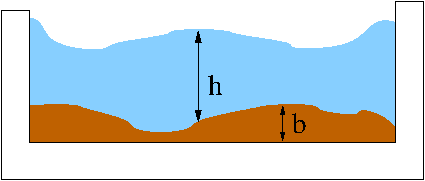
\includegraphics{basin_bathy}}
\end{DoxyImageNoCaption}
 

The shallow water equations describe the changes of water depth {\itshape h} and horizontal velocities {\itshape v$_{\mbox{x}}$ } and {\itshape v$_{\mbox{y}}$ } (in the resp. coordinate directions) over time, depending on some initial conditions -- in the case of tsunami simulation, these initial conditions could, for example, result from an initial elevation of the sea floor caused by an earthquake. The respective changes in time can be described via a system of partial differential equations\-: \[ \begin{array}{c} \displaystyle \frac{\partial h}{\partial t} + \frac{\partial (v_x h)}{\partial x} + \frac{\partial (v_y h)}{\partial y} = 0 \\[1em] \displaystyle \frac{\partial (h v_x)}{\partial t} + \frac{\partial (h v_x v_x)}{\partial x} + \frac{\partial (h v_y v_x)}{\partial y} + \frac{1}{2} g \frac{\partial (h^2)}{\partial x} = - gh \frac{\partial b}{\partial x}, \\[1em] \displaystyle \frac{\partial (h v_y)}{\partial t} + \frac{\partial (h v_x v_y)}{\partial x} + \frac{\partial (h v_y v_y)}{\partial y} + \frac{1}{2} g \frac{\partial (h^2)}{\partial y} = - gh \frac{\partial b}{\partial y}, \end{array} \] The equation for {\itshape h} is obtained, if we examine the conservation of mass in a control volume. The equations for {\itshape hv$_{\mbox{x}}$ } and {\itshape hv$_{\mbox{y}}$ } result from conservation of momentum (note that {\itshape h} is directly related to the volume, and thus the mass of the water -- thus {\itshape hv$_{\mbox{x}}$ } can be interpreted as a momentum).

The two terms involving {\itshape g} model a gravity-\/induced force ({\itshape g} being the constant for the gravitational acceleration, {\itshape g} = 9.\-81 ms$^{\mbox{-\/2}}$ ), which results from the hydrostatic pressure. The right-\/hand-\/side source terms model the effect of an uneven ocean floor ({\itshape b} obtained from respective bathymetry data).\hypertarget{index_finvol}{}\subsection{Finite Volume Discretisation}\label{index_finvol}
The shallow water equations are usually too difficult to be solved exactly -\/ hence, S\-W\-E implements simple discrete models as an approximation. As the applied numerical method (typically a Finite Volume discretization) may vary, we will stick to the basics at this point.

First, S\-W\-E assumes that the unknown functions {\itshape h(t,x,y)}, {\itshape hu(t,x,y) \-:= h(t,x,y) v$_{\mbox{x}}$ (t,x,y)}, {\itshape hv(t,x,y) \-:= h(t,x,y) v$_{\mbox{y}}$ (t,x,y)}, as well as the given sea bottom level {\itshape b(x,y)}, are approximated on a Cartesian mesh of grid cells, as illustrated below. In each grid cell, with indices {\itshape (i,j)}, the unknowns have constant values {\itshape h$_{\mbox{ij}}$ }, {\itshape hu$_{\mbox{ij}}$ }, {\itshape hv$_{\mbox{ij}}$ }, and {\itshape b$_{\mbox{ij}}$ }\-:

 
\begin{DoxyImageNoCaption}
  \mbox{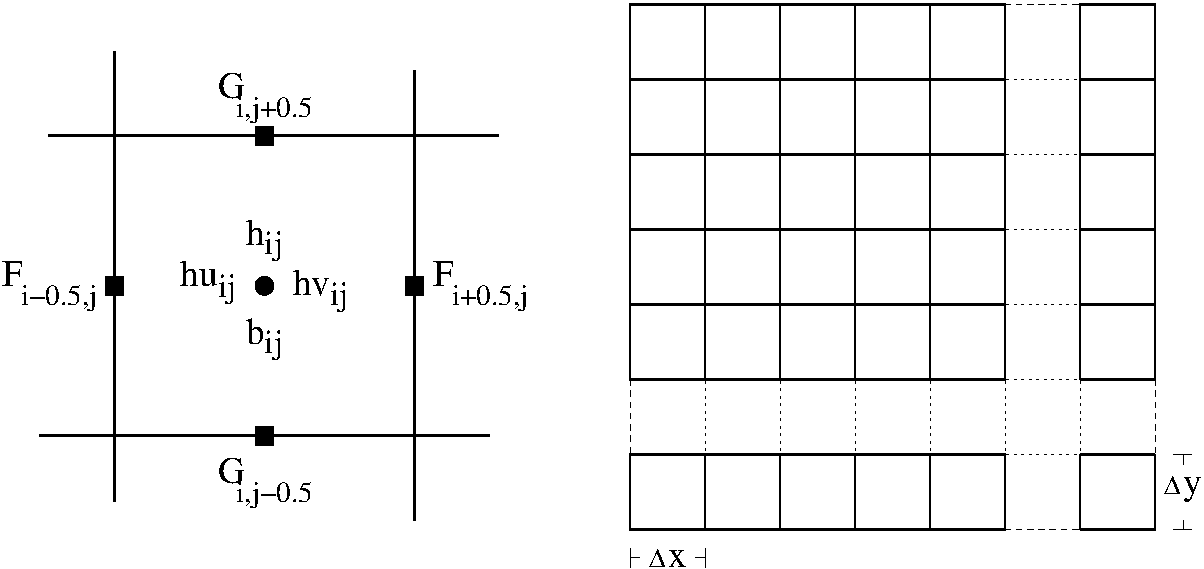
\includegraphics{grid_unknowns}}
\end{DoxyImageNoCaption}
\hypertarget{index_fluxes}{}\subsection{Computing Numerical Fluxes at Edges and Euler Time-\/\-Stepping}\label{index_fluxes}
The details of the numerical schemes are too complicated to be described in this overview. Please refer to the accompanying material. To put it short, we successively perform two main computational steps\-:
\begin{DoxyItemize}
\item we compute so-\/called {\bfseries numerical fluxes} on each edge of the grid (which approximate the transfer of mass or momentum between grid cells),
\item based on these numerical fluxes, we then update the unknowns in each cell.
\end{DoxyItemize}\hypertarget{index_impl}{}\section{Implementation and base class S\-W\-E\-\_\-\-Block}\label{index_impl}
For the simulation of the shallow water model, we thus require a regular Cartesian grid, where each grid cell carries the respective unknowns -\/ water level, momentum in x-\/ and y-\/direction, and bathymetry data. The central data structures for Cartesian grid and arrays of unknowns are provided with the abstract base class \hyperlink{classSWE__Block}{S\-W\-E\-\_\-\-Block}, which has four 2\-D arrays \hyperlink{classSWE__Block_a64a0f8f437f38b5f3b8ec5b4abdb864e}{S\-W\-E\-\_\-\-Block\-::h}, \hyperlink{classSWE__Block_aec2c1278fdb23f083216d8d397f26060}{S\-W\-E\-\_\-\-Block\-::hu}, \hyperlink{classSWE__Block_a0897aa3c2d78749f209c95e08196d831}{S\-W\-E\-\_\-\-Block\-::hv}, and \hyperlink{classSWE__Block_af7487209129f40b26ea171762754a261}{S\-W\-E\-\_\-\-Block\-::b}. To implement the behaviour of the fluid at boundaries, and also to allow the connection of several grid blocks (for parallelization or just to build more complicated computational domains), each array has an additional layer of so-\/called {\itshape ghost cells}, as illustrated in the following figure\-:


\begin{DoxyImageNoCaption}
  \mbox{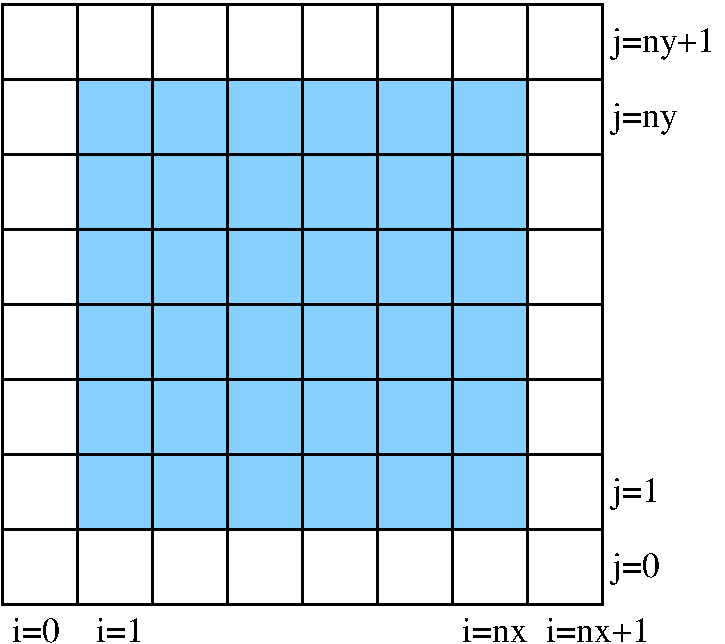
\includegraphics{ghost_cells}}
\end{DoxyImageNoCaption}
 \hypertarget{index_models}{}\subsection{Parallelisation and Different Models}\label{index_models}
In each time step, our numerical algorithm will compute the flux terms for each edge of the computational domain. To compute the fluxes, we require the values of the unknowns in both adjacent cells. At the boundaries of the fluid domain, the ghost layer makes sure that we also have two adjacent cells for the cell edges on the domain boundary. The values in the ghost layer cells will be set to values depending on the values in the adjacent fluid domain. We will model three different situations\-: \{description\} \{Outflow\-:\} \{h\}, \{u\}, and \{v\} in the ghost cell are set to the same value as in the adjacent fluid cell. This models the situation that the unknowns do not change across the domain boundary (undisturbed outflow). \{Wall\-:\} At a wall, the velocity component normal to the boundary should be \$0\$, such that no fluid can cross the boundary. To model this case, we set the normal velocity, e.\-g. \{u\mbox{[}0\mbox{]}\} at the left boundary, to the negative value of the adjacent cell\-: \{-\/u\mbox{[}1\mbox{]}\}. The interpolated value at the boundary edge will then be \$0\$ (\{h\} is identical in both cells due to the imposed boundary condition). The other two variables are set in the same way as for the outflow situation. \{Connect\-:\} With the connect case, we can connect a domain at two boundaries. If we connect the left and right boundary, we will obtain a periodically repeated domain. Here, all ghost values are determined by the values of the unknowns in the fluid cell adjacent to the connected boundary. \{description\}

To implement the boundary conditions, the class \{\hyperlink{classSWE__Block}{S\-W\-E\-\_\-\-Block}\} contains an array of four enum variables, \{boundary\mbox{[}4\mbox{]}\} (for left/right/bottom/top boundary), that can take the values {\ttfamily O\-U\-T\-F\-L\-O\-W}, {\ttfamily W\-A\-L\-L}, and {\ttfamily C\-O\-N\-N\-E\-C\-T}.\hypertarget{index_multblocks}{}\subsection{Multiple Blocks}\label{index_multblocks}
Via the connect boundary condition, it is also possible to connect several Cartesian grid blocks to build a more complicated domain. Figure fig\-:connect\} illustrates the exchange of ghost values for two connected blocks.

  
\begin{figure}
\begin{center}
  \includegraphics[width=0.8\textwidth]{pics/connect.pdf}
\end{center}
\caption{Exchange of values in ghost layers between two connected \texttt{SWE\_Block}s.}
\label{fig:connect}
\end{figure}


To store the neighbour block in case of a {\ttfamily C\-O\-N\-N\-E\-C\-T} boundary, {\ttfamily \hyperlink{classSWE__Block}{S\-W\-E\-\_\-\-Block}} contains a further array of four pointers, {\ttfamily neighbour\mbox{[}4\mbox{]}} (for left/right/bottom/top boundary), that will store a pointer to the connected adjacent {\ttfamily \hyperlink{classSWE__Block}{S\-W\-E\-\_\-\-Block}}.

The respective block approach can also be exploited for parallelisation\-: the different blocks would then be assigned to the available processors (or processor cores) -- each processor (core) works on its share of blocks, while the program has to make sure to keep the values in the ghost cells up to date (which requires explicit communication in the case of distributed-\/memory computers).\hypertarget{_}{}\subsection{}\label{_}
For each time step, our solver thus performs the following steps -- each step is implemented via a separate member function of the class \{\hyperlink{classSWE__Block}{S\-W\-E\-\_\-\-Block}\}\-: \{enumerate\}  set the values at the boundaries\-: \{set\-Boundary\-Layer()\};  compute the flux terms for all edges\-: \{compute\-Fluxes()\};  from the flux terms, compute the in/outflow balance for each cell, and compute the new values of the unknowns for the next time step\-: \{euler\-Timestep()\}. \{enumerate\}\hypertarget{_}{}\subsection{}\label{_}
The class \{\hyperlink{classSWE__Block}{S\-W\-E\-\_\-\-Block}\} contains further methods that will write the numerical solution into a sequence of files that can be read by the visualisation package Para\-View (just enter the respective folder from Para\-View -- the files will be recognised and displayed as one project). Para\-View allows to visualise the computed time-\/dependent solution (as ``movie'' or in single-\/step mode). Para\-View is pretty self-\/explanatory for our purposes, but provides an online help for further instructions.\hypertarget{_}{}\subsection{}\label{_}
We also provide a C\-U\-D\-A implementation of the simulation code (requires a computer with a C\-U\-D\-A-\/capable G\-P\-U, together with the respective drivers -- visit N\-V\-I\-D\-I\-A's website on C\-U\-D\-A for details on implementation). Apart from the fact that the simulation usually runs a lot faster on the G\-P\-U, the program is also capable of plotting the computing solution (water surface) ``on the fly''.

Finally\-: whoever thinks that they can do a better (faster, ...) implementation (visualisation, ...) of the provided code is more than welcome to do so! Feel free to contribute to S\-W\-E -\/ for questions, just contact Michael Bader (\href{mailto:bader@in.tum.de}{\tt bader@in.\-tum.\-de}). 